% Hier bitte ausfüllen:
\newcommand{\praktikum}{} % Praktikum P3/P4
\newcommand{\gruppennummer}{} % Gruppennummer
\newcommand{\gruppentag}{} % Gruppentag
\newcommand{\semester}{} % Semester
\newcommand{\versuch}{} % Versuch
\newcommand{\nameeins}{} % Name1 (Vor und Nachname)
\newcommand{\emaileins}{} % E-Mail 1
\newcommand{\namezwei}{} % Name2 (Vor und Nachname)
\newcommand{\emailzwei}{} % E-Mail 2
\newcommand{\assistent}{} % Assistent:in
\newcommand{\durchfuehrungsdatum}{} % Durchgeführt am
\newcommand{\abgabedatum}{} % Protokollabgabe am:
%%%%%%%%%%%%%%%%%%%%%%%%%%%%%%%%%%%%%%%%%%%%%%%%%%%%%%%%%%%%%%%%%%%%%%%%%%%%%%%%%%%%%%%%%
\begin{tikzpicture}[remember picture,overlay]
    \node at (current page.center) {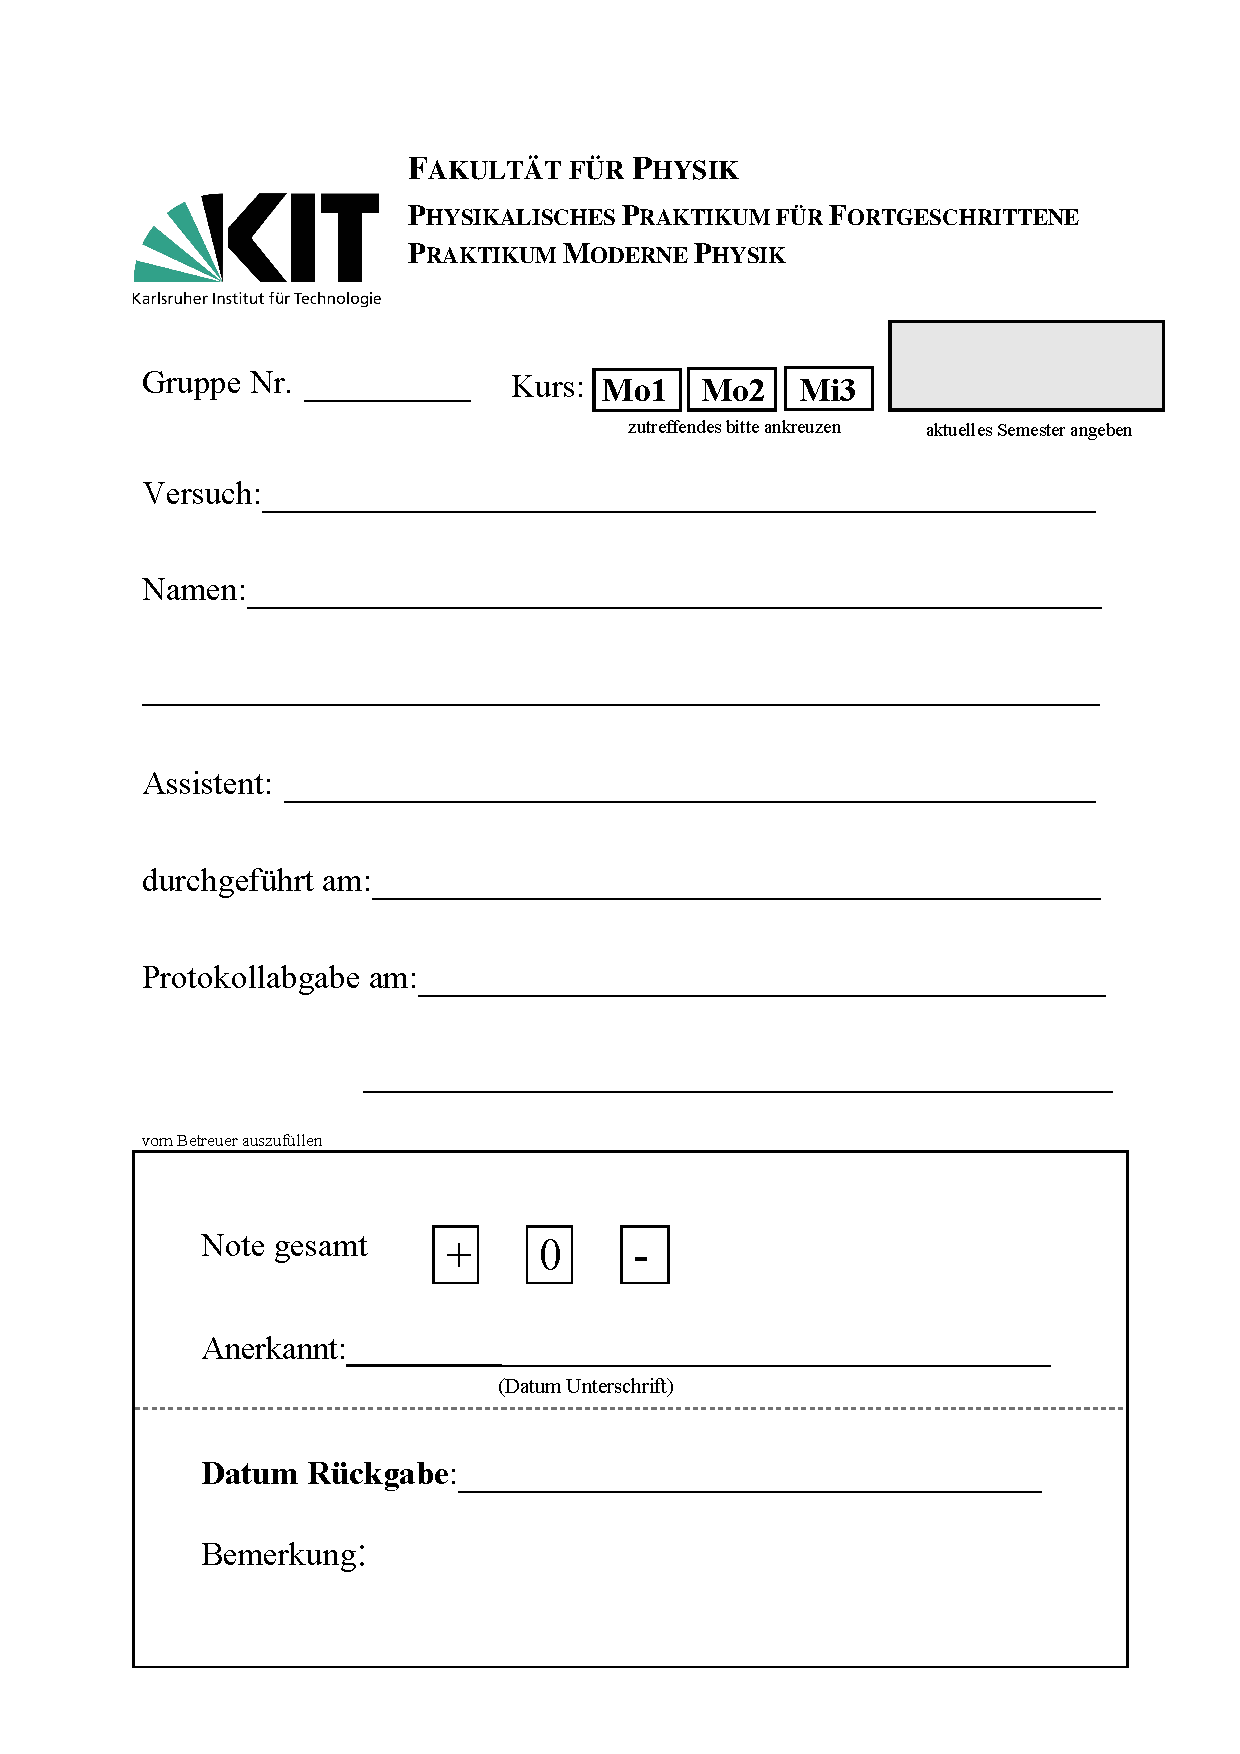
\includegraphics[page=1]{include/DeckblattP3P4.pdf}};
    \begin{scope}[shift={(current page.south west)},every node/.style={anchor=base west}]
        % Grid to help find the positions (remove in final version)
        %\draw [help lines] (0,0) grid (current page.north east);
        %\draw [help lines,thick] (0,0) grid [step=5cm] (current page.north east);
        % Gruppennummer:
        \node at (5.8cm,23.1cm){\Large{\gruppennummer}};
        %Bitte richtigen Wochentag angeben
        %\node at (10 cm,22.8cm) {\scalebox{4}{{$\mathbf{\times}$}}}; % Mo1 Gruppentag:
        %\node at (11.7cm,22.8cm) {\scalebox{4}{{$\mathbf{\times}$}}}; % Mo2 Gruppentag:
        %\node at (13.3 cm,22.8cm) {\scalebox{4}{{$\mathbf{\times}$}}}; % Mi3 Gruppentag:
        \node at (16cm,23.1cm) {\Large{\semester}}; % Semester:
        \node at (4.8cm,21.2cm){\Large{\versuch}}; %Versuch:
        \node at (4.8cm,19.6cm){\Large{\nameeins\hspace{0.2222em}(\emaileins)}}; % Name 1.Zeile:
        \node at (4.8cm,18.0cm){\Large{\namezwei\hspace{0.2222em}(\emailzwei)}}; % Name 2.Zeile:
        \node at (4.8cm,16.3cm){\Large{\assistent}}; % Assistent:in:
        \node at (7.2cm,14.6cm){\Large{\durchfuehrungsdatum}}; % durchgeführt am:
        \node at (7.2cm,13.0cm){\Large{\abgabedatum}}; % Protokollabgabe am:
    \end{scope}
\end{tikzpicture}
% This information will appear embed into the PDF file as meta data
\hypersetup{
  pdftitle    = {\praktikum\hspace{0.2222em}Protokoll - \versuch},
  pdfsubject  = {Protokoll des Versuchs \versuch\hspace{0.2222em}vom \durchfuehrungsdatum},
  pdfauthor   = {\nameeins\hspace{0.2222em}und\hspace{0.2222em}\namezwei\hspace{0.2222em}(Gruppe \gruppentag-\gruppennummer)},
  pdfkeywords = {KIT, Physik, Praktikum, Protokoll, \praktikum, \versuch, \semester, \nameeins, \namezwei},
  pdfcreator  = {pdflatex},
  pdfproducer = {LaTeX with hyperref}
}